\documentclass[12pt, unicode]{beamer}
\usetheme{CambridgeUS}
\usepackage{luatexja, xcolor}

\title{Introduction to Ants}
\author{\textcolor[HTML]{804000}{harry\_arbrebleu}}
\date{\today}
\institute[慶應理工]{慶應義塾大学理工学部}
\begin{document}
  \frame{\maketitle}
  \begin{frame}{自己紹介}
    \begin{description}
      \item[名前] \textcolor[HTML]{804000}{harry\_arbrebleu},青木陽(Haruki Aoki) \pause
      \item[学部,学年] 理工学部物理情報工学科,B2
      \item[趣味] 競プロ(10月から),\LaTeX,写真,ロードバイク,読書,宇多田ヒカル
      \item[書ける言語(程度は問わない)] Japanese,English,French,Python,C++
    \end{description}
  \end{frame}
  \begin{frame}
    \begin{figure}
      \centering
      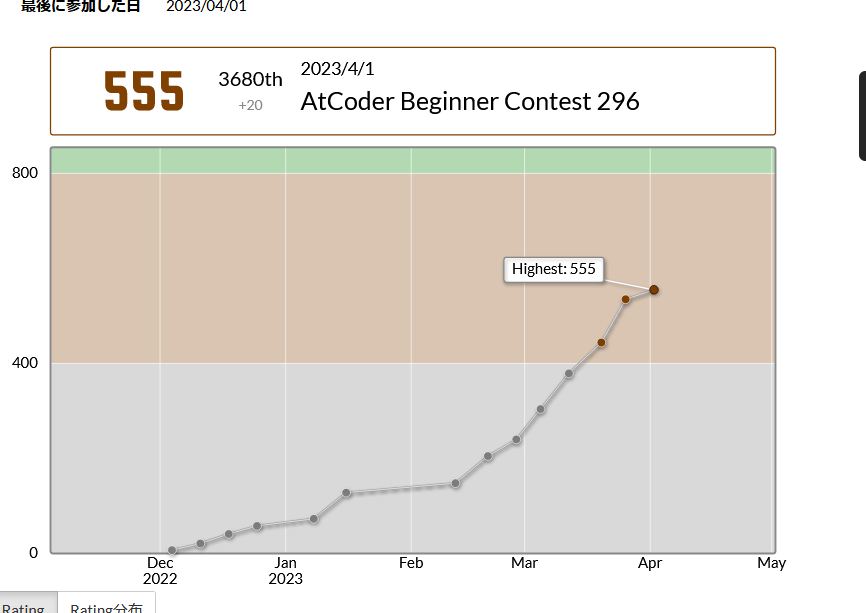
\includegraphics[scale = 0.5]{progression.png}
    \end{figure}
  \end{frame}
  \begin{frame}
    \begin{figure}
      \centering
      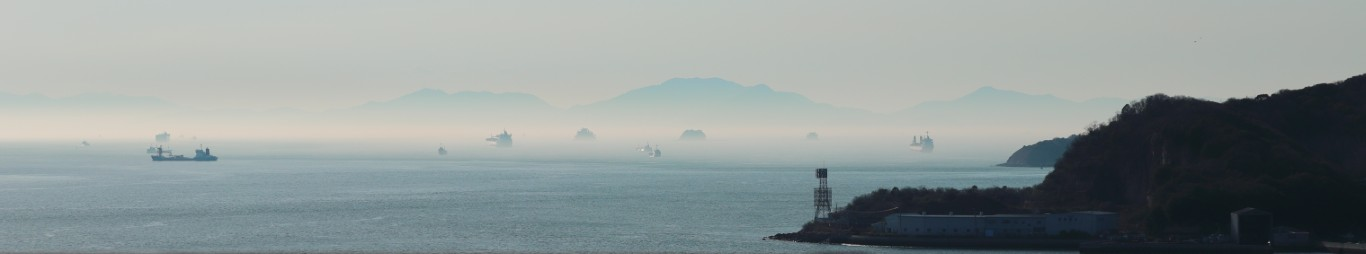
\includegraphics[scale = 1]{my_photo.JPG}
    \end{figure}
  \end{frame}
  \begin{frame}{そもそもこの団体は?}
    \begin{itemize}
      \item \textcolor[HTML]{c0c000}{momoyuu},\textcolor[HTML]{008000}{rafi2}と一緒に設立しました! \pause
      \item この間(2023/4/3)未公認団体となった学生団体です.\pause
      \item ICPC, WFを目指して活動します. 
      \item アルゴリズムがメインですが,将来的にはヒューリスティックやKaggleにも手を伸ばしたいと考えています.
    \end{itemize}
  \end{frame}
  \begin{frame}{今のところどんな人が興味を持っているの?(1/3)}
    \begin{figure}
      \centering
      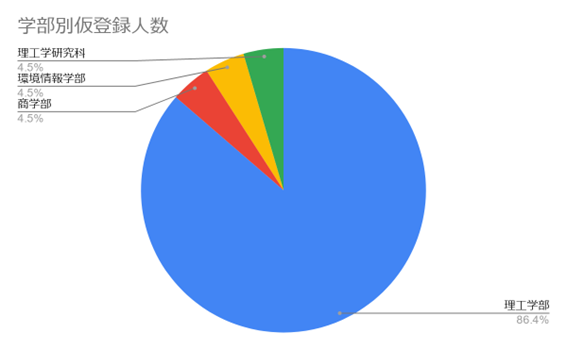
\includegraphics[scale = 0.5]{faclty.png}
    \end{figure}
  \end{frame}
  \begin{frame}{今のところどんな人が興味を持っているの?(2/3)}
    \begin{figure}
      \centering
      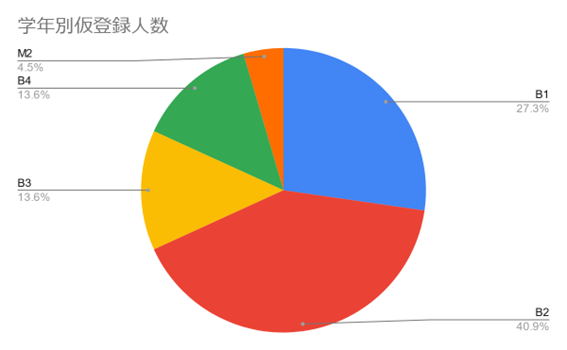
\includegraphics[scale = 0.5]{year.png}
    \end{figure}
  \end{frame}
  \begin{frame}{今のところどんな人が興味を持っているの?(3/3)}
    \begin{figure}
      \centering
      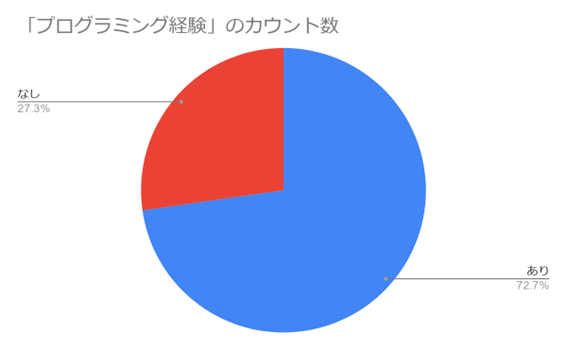
\includegraphics[scale = 0.5]{experience.png}
    \end{figure}
  \end{frame}
  \begin{frame}{input系の活動}
    \begin{block}{定期活動}
      \begin{description}
        \item[全員] バチャ週1回$\rightarrow$解説 \pause
        \item[初心者] AICセミナーのフォローアップ \pause
        \item[初心者,中級者] 鉄則本の輪読 (講師: \textcolor[HTML]{008000}{rafi2})
        \item[中級者から] 蟻本の輪読(講師: \textcolor[HTML]{c0c000}{momoyuu}) \pause
      \end{description}
    \end{block}
    \begin{exampleblock}{不定期活動}
      \begin{description}
        \item[全員向け] ABC解説,解法共有 \pause
        \item[全員向け] アルゴリズム勉強会(高度典型など) 
      \end{description}
    \end{exampleblock}
  \end{frame}
  \begin{frame}{output系の活動}
    \begin{block}{定期活動}
      \begin{description}
        \item[全員向け] AtCoder Problemsのバーチャルコンテスト \pause
      \end{description}
    \end{block}
    \begin{exampleblock}{不定期活動}
      \begin{itemize}
        \item Codeforcesのバーチャルコンテスト \pause
        \item ICPC向けの5hバーチャルコンテスト
      \end{itemize}
    \end{exampleblock}
  \end{frame}
  \begin{frame}{Antsで出来ること}
    \begin{enumerate}
      \item 競技プログラミングを一緒にやる仲間を作れる.\pause
      \item 何か分からないことがあったらすぐに聞ける. \pause
      \item お互いに教え合いながら,実力が向上できる.\pause
      \item ICPCのチームを作れる.
    \end{enumerate}
  \end{frame}
  \begin{frame}{今後の流れ}
    \begin{enumerate}
      \item 親睦会を開催します.この後,\textbf{ABCに間に合うように}ごはん行きましょう. \pause
      \item 今後に活用するのでアンケートの入力をお願いします!
    \end{enumerate}
  \end{frame}
  \frame{\centering \Large Thank you for your large attention!!}
\end{document}
